\documentclass[twocolumn]{article}
\usepackage[utf8]{inputenc}
\usepackage[english]{babel}
\usepackage{abstract}
\usepackage{booktabs}

\usepackage{siunitx}    
\usepackage{makecell}

\usepackage{hyperref}


\usepackage[
backend=biber,
style=alphabetic
]{biblatex}
\addbibresource{references.bib}


\usepackage{graphicx}
\graphicspath{ {latexIMG/} }


\title{\textbf{AML Project}
\\Federated Learning: where machine learning \\and data privacy can coexist
}

\author{
Alfredo Baldó Chamorro | 
Bastien Bertholom |
Giuseppe Salvi
}
\date{13 February 2022}

\begin{document}


\maketitle

\section{Abstract}
With the mass of data generated each day by multiple sources (i.e. IoT), machine learning has a bright future. Unfortunately, a huge part of this data is not usable due to their private nature regarding users. Federated learning is a machine learning framework aiming to guarantee this privacy by keeping the data locally on the device (i.e. mobile phones).
\section{Introduction} %mandatory

Introduced by Google in 2016 \cite{DBLP:journals/corr/KonecnyMYRSB16}, Federated Learning enables models to be iteratively trained in a decentralized way, on local devices. At each round, a subset of sources (also called \emph{clients}) are selected to perform local training on their own data. Then, the centralized model aggregates the ensemble of updates to make the new global model and send back it to another subset of clients. 

As a part of the Advanced Machine Learning course at Politecnico di Torino, this paper will cover the work on the replication of the experiment proposed by \cite{DBLP:journals/corr/abs-2003-08082} on the CIFAR10 dataset which consists of analyzing the effects that client's data distributions have on federated models. Especially distributions such as Non-Identical Class Distribution (each client has a different class distribution) and Imbalanced Client Sizes (each client has a different amount of data). 

The work will cover the federated scenario using the standard FedAvg algorithm with multiple sets of parameters and evaluate the one with the greatest performance. Experiments with different settings such as data distribution, normalization layers and group normalization will be implemented. Finally, there will be a solution proposal (which will be a test) in order to solve one of the identified problems.

\section{Related Work} %mandatory
This experiment has already been performed by \cite{DBLP:journals/corr/abs-2003-08082}  on the iNaturalist-2017 dataset. They provided an analysis of the effect of learning with per-user data and proposed two new algorithms (FedVC, FedIR) and provided new large-scale datasets with per-user data.

A different algorithm (FedAvgM) has been proposed by \cite{DBLP:journals/corr/abs-1909-06335} using momentum on top of SGD to accelerate the network training. This approach changes the way the weights are updated to add momentum at the server side.

\section{Methods} %mandatory describe algorithms
There are various steps in the building of the final algorithm. In this section the decisions that led to choose the values for the parameters and the choice for different algorithms implemented will be explained. 

Federated learning applied in the real world, would take into account multiple devices with different characteristics (CPU capacity and speed...). The model and algorithm selection was chosen on the basis of a hypothetical implementation on different devices.  

\subsection{Problem setup}
Federated Learning consists of a client and a server side. Considering the CIFAR10 dataset contains 50000 samples for training and 10000 samples for testing, choosing the number of clients K = 100 was thought as to be representing of a real-world scenario (averaging 500 images per client for training). 

Moreover, in order to simulate real world data, a Delta variable was implemented into the code in order to add randomness regarding the distribution of the data among clients. The variable added some casualty to the quantity of data that each client would be seeing. For example, if Delta = 100, each of the 100 clients would have data between a minimum of 400 images and a maximum of 600. (50 000 / 100 = 500 +- 100).


To add up, the distribution of data was considered to be performed randomly. The variability Delta introduced was not substantial, and this was done intentionally. The problem of some client having way bigger amount of images than others (2-3 times) could have been solved with the creation of additional virtual clients and splitting the data among them. In terms of implementation this would be equal to increasing the number of clients from K to K + i, where i is the number of the virtual clients created. 

Moreover in order to test the model, the accuracy on the training was computed as an average of the accuracy on the client's data. On the validation part, the accuracy was tested with the whole validation dataset on the server side.

Finally the number of clients C, was chosen based on performance. As the table \ref{table:CComp}, relates, the best performance is for C=0.4, however the number of clients increases significantly and hence computational time. For this reason, the next best value of C (C=0.3) was chosen for the model.


\begin{table}
\centering
\begin{tabular}{||c c ||} 
  \toprule
    \makecell{C Values} &\makecell{Validation Accuracy (\%)} \\
  \midrule
  0.1  & 54,91  \\
 \hline
 0.2 & 64,96 \\
 \hline
  0.3 &  69,79 \\
 \hline
  0.4 & \ensuremath{\mathbf{73,12}} \\
  \bottomrule                             
\end{tabular}
\caption{Performance comparison with different C values}
\label{table:CComp}
\end{table}


\subsection{Network}

With that in mind, for the neural network, a variation of LeNet5 was chosen, which has two 5×5, 64-channel convolution layers, each precedes a 2×2 max-pooling layer, followed by two fully-connected layers with 384 and 192 channels respectively and finally a softmax linear classifier \cite{DBLP:journals/corr/abs-2003-08082}. 

As each device implements the model and considering each having a different computational capacity, a small and simple network was selected in order for the computation to be the quickest possible but also having the capacity to gather information from the client's dataset.

\subsection{Algorithm}
The Federated Average algorithm (FedAvg) was picked for the sever aggregation part of the algorithm. The FedAvg consists on aggregating the weights of the clients according the number of images each client sees, with respect to the total number of images of the dataset.
The FedAvg algorithm is simple, but useful enough in order to get an acceptable accuracy.

In addition, a variant of the Federated Average algorithm with server momentum was also considered, called FedAvgMomentum \cite{DBLP:journals/corr/abs-1909-06335}. Vanilla FedAvg updates the weights via: \[ w \leftarrow w - \Delta  w\] where \[\Delta  w  \] is the weighted average of the weight updates of the clients. To add momentum at the server side, a different computation is made instead \[ \nu \leftarrow  \beta\nu + \Delta w  \] and update the model with: \[w \leftarrow w - \nu \]

A comparison between the two algorithms was thought as interesting in order to see what impact the introduction of the momentum server had on the speed of convergence and oscillations, particularly in the scenario where clients have different data distributions.


\section{Experiments} % mandatory
\subsection{Federated Average}
As baseline model, Federated Average (FedAvg) algorithm was chosen. In order to get an idea of the performance of the algorithm, a comparison with the centralised model was needed. 

First of all, fine-tuning the parameters for the centralized model was necessary. A decision was made to adopt the number of epochs E = 100, as a trade off between performance and computational cost. The best learning rate the value LR = 2e-3 was discovered as resulting in better performance, because lower values had worse results, while higher values showed overfitting. With that in mind, in the federated model, the same learning rate was used, and a decision was made to use 20 rounds of 5 local epochs, to have a fair comparison between the two scenarios.

** In the plots from the federated experiments, the term epoch refers to rounds and not to local epochs. **

Figure \ref{AccCompFedCent} represents the difference in performance between centralised and federated model with different set configuration. It's evident and as awaited, that the centralised model has a better performance in all scenarios. The FedAvg does not lead to a good accuracy, hardly reaching 70\%. Still, being a model without any further optimization, the accuracy was thought as acceptable.


\begin{figure}
    \centering
    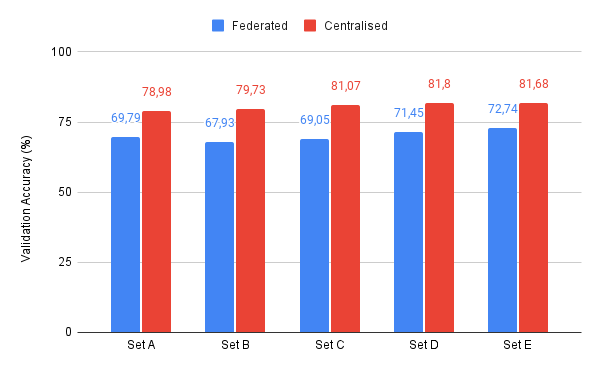
\includegraphics[width=0.5\textwidth,height=.3\textheight]{FedAccuracyComp.png}
    \caption{Accuracy comparison between centralised and federated model. (Set A: no normalization, Set B: batch normalization, Set C: group normalization (2-2), Set D: group normalization (2-4), Set C: group normalization (2-16)}
     \label{AccCompFedCent} 
\end{figure}
\subsection{Group and Batch Normalization}
In order to be able to decide which model implementation is better, a comparison between normalization was made in table \ref{batchNormComp}. What can be extracted from this experiment is that normalization is relevant for the accuracy. It's true that the accuracy decreases in the federated model by adding batch normalization (from 69,79 to 67,93 \% for no normalization and batch normalization respectively). However, normalization seems crucial as adding group normalization added up to 4\% in accuracy performance. 


\begin{table}
\centering
\begin{tabular}{||c c c||} 
  \toprule
 \makecell{Model} & \makecell{Validation \\Accuracy (\%)} & \makecell{Normalization}  \\
  \midrule
  Federated  & 67,93 & Batch \\
 \hline
 Federated & 69,79 & No\\
 \hline
  Federated &  \ensuremath{\mathbf{73,15}} & \makecell{Group (8-2)}\\
 \hline
  Centralised & 79,73 & Batch\\
   \hline
  Centralised  & 78,98  & No\\
   \hline
  Centralised  & \ensuremath{\mathbf{81,7}} & Group\\
  \bottomrule                             
\end{tabular}
\caption{Performance comparison with batch normalization for 10 rounds and 10 epochs}
\label{batchNormComp}
\end{table}


\subsection{Different data sizes}
In order to simulate different quantity of data that each client is going to have, a variable Delta was implemented in order to add randomness. The experiment was followed by changing the number of groups division of the group normalization layer 1 and 2. The results are represented in figure \ref{AccDiff}, illustrating with different group normalization parameters, the accuracy over the validation set. 

Sticking with figure \ref{AccDiff}, over 8 tests done, there's no clear difference of a better performance with or without Delta variable. Therefore, a new experiment was done, however this one just varying Delta to see the behaviour of the model, anything else remained unchanged. The results are presented in figure \ref{DeltaValue}. As it can be seen from the graph, for a Delta varying from 50 to 300 the accuracy does not decrease, however, after Delta =400, it appears as the performance starts to decrease which was expected (from 73,44\% to 70,64\%), as the data among the clients start to differ substantially.


\begin{figure}
    \centering
    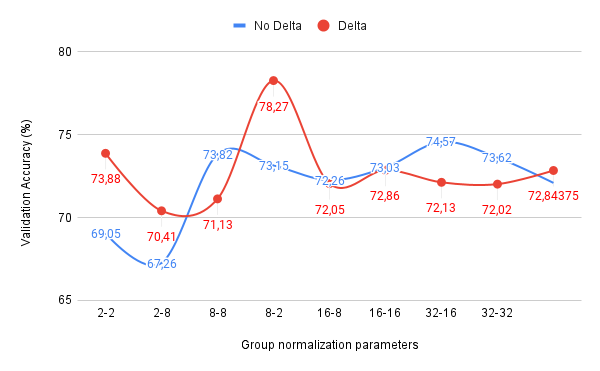
\includegraphics[width=0.5\textwidth,height=.3\textheight]{groupnormalizationDeltaNoDelta.png}
    \caption{Accuracy over validation set with Delta = 100 variable activated or not}
     \label{AccDiff} 
\end{figure}

\begin{figure}
    \centering
    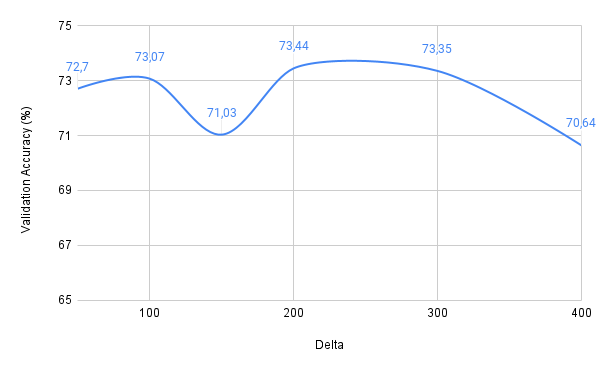
\includegraphics[width=0.5\textwidth,height=.3\textheight]{deltacomparison.png}
    \caption{Accuracy over validation set with different Delta values variable}
     \label{DeltaValue} 
\end{figure}

\subsection{Dirichlet distribution}

In order to achieve a better understanding of the possible accuracy outcomes when deploying the model, different data distribution between clients should be taken into account. In order to simulate client getting different data distribution, the Dirichlet distribution was used. The parameter Alpha, represents how different the distribution is between clients: with a greater Alpha, the distributions 
would be similar, with smaller Alpha, the distribution between clients differs.
In particular, when Alpha is equal to 0 each client has access to data belonging to only one class.

In order to implement it, data already distributed with different Alpha parameters was taken from \url{https://github.com/google-research/google-research/tree/master/federated_vision_datasets} where Alpha goes from 0 to 100 for the CIFAR10 dataset.



The results are shown in figure \ref{AccAlpha}. This image clearly illustrates the fact that expanding the difference in the dataset distribution between clients (lower Alpha), as expected, leads to the decrease in accuracy. 
Moreover, from the plots of training and validation accuracy ( Figure \ref{AccFedAvgA1}, Figure \ref{AccFedAvgA10}, Figure \ref{AccFedAvgA100} ), it can be seen how the smaller Alpha, the greater the number of oscillations.
The accuracy on the training is higher because the smaller the Alpha, the smaller the number of classes each clients gets, hence a perfect prediction is expected. 

\begin{figure}
    \centering
    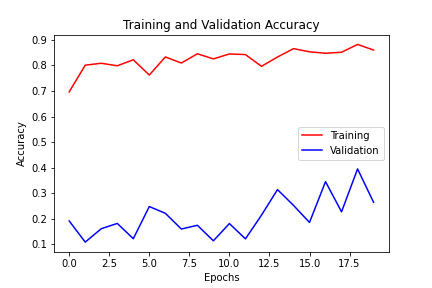
\includegraphics[width=0.5\textwidth,height=.3\textheight]{2_AccuracyFedAvg_A1.png}
    \caption{Accuracy using FedAvg with Alpha = 1}
     \label{AccFedAvgA1} 
\end{figure}

\begin{figure}
    \centering
    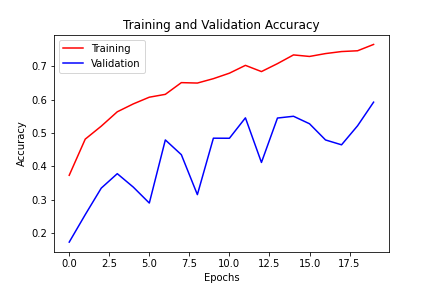
\includegraphics[width=0.5\textwidth,height=.3\textheight]{2_AccuracyFedAvg_A10.png}
    \caption{Accuracy using FedAvg with Alpha = 10}
     \label{AccFedAvgA10} 
\end{figure}

\begin{figure}
    \centering
    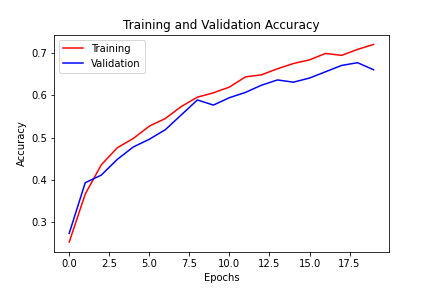
\includegraphics[width=0.5\textwidth,height=.3\textheight]{2_AccuracyFedAvg_A100.png}
    \caption{Accuracy using FedAvg with Alpha = 100}
     \label{AccFedAvgA100} 
\end{figure}

To obtain results that are more similar to the IID scenario also for lower values of Alpha, increasing a lot the number of communication rounds was needed. For example, in Figure \ref{AccA1R200} with Alpha = 1 validation accuracy reaches around 65\% accuracy after 200 rounds like in the IID setting.
\begin{figure}
    \centering
    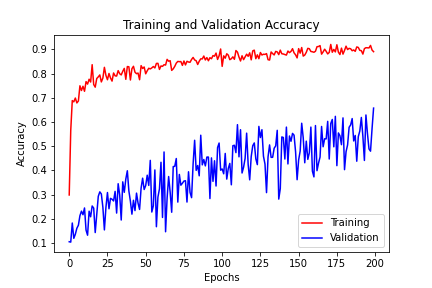
\includegraphics[width=0.5\textwidth,height=.3\textheight]{3_AccuracyFedAvg_A1R200.png}
    \caption{Accuracy with Alpha = 1}
    \label{AccA1R200} 
\end{figure}

Finally, the figure \ref{AccAlpha} states that the group normalization model over-performs the model without normalization. This behavior goes along with the results gotten in the normalization experiments, and in this situation, normalization has an even more important role.


\begin{figure}
    \centering
    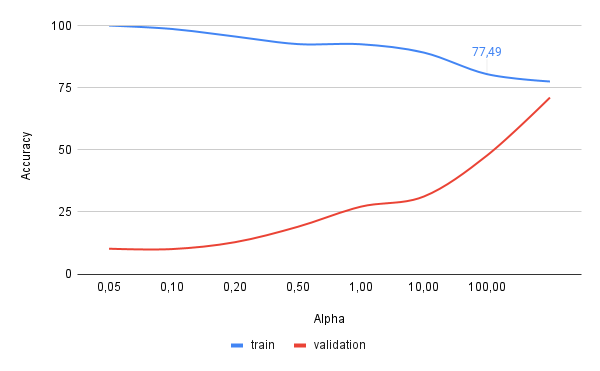
\includegraphics[width=0.5\textwidth,height=.3\textheight]{alphaAccuracy.png}
    \caption{Accuracy over different values of Alpha}
    \label{AccAlpha} 
\end{figure}


\subsection{Federated Average Momentum (additional contribution)}

The same setup of the previous experiments (Rounds = 20, Epochs = 5, Local Batch size = 32, K = 100, C = 0.3) is taken as starting point for the analysis.
For the FedAvgM the same settings as in [REFERENCE FOR PAPER] was used: SGD as the optimizer for the server model,  momentum (beta) = 0.9, and centralised model learning rate fixed to 1.
From the accuracy and loss plots (\ref{AccFedAvgIid}, \ref{LossFedAvgIid}, \ref{AccFedAvgMIid}, \ref{LossFedAvgMIid}) with IID data distributions for the clients, it can be seen how the results are very similar. However, the solution with server momentum has smaller oscillations and converges slightly faster. 

\begin{figure}
    \centering
    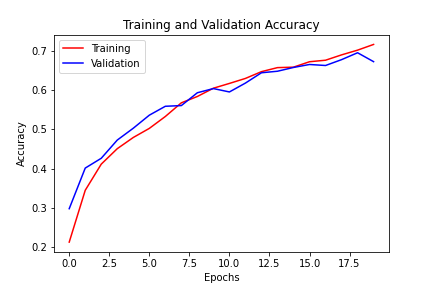
\includegraphics[width=0.5\textwidth,height=.3\textheight]{4_AccuracyFedAvg_iid.png}
    \caption{Accuracy using FedAvg with iid data distributions}
     \label{AccFedAvgIid} 
\end{figure}

\begin{figure}
    \centering
    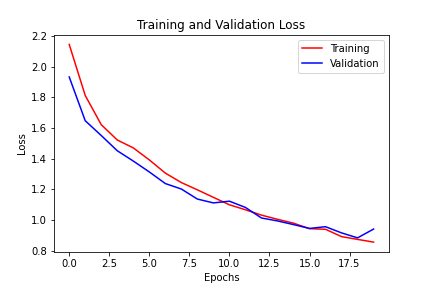
\includegraphics[width=0.5\textwidth,height=.3\textheight]{4_LossFedAvg_iid.png}
    \caption{Loss using FedAvg with iid data distributions}
     \label{LossFedAvgIid} 
\end{figure}

\begin{figure}
    \centering
    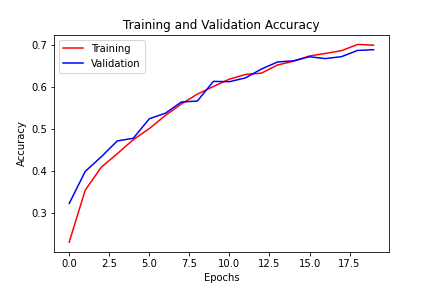
\includegraphics[width=0.5\textwidth,height=.3\textheight]{4_AccuracyFedAvgM_iid.png}
    \caption{Accuracy using FedAvgM with iid data distributions}
     \label{AccFedAvgMIid} 
\end{figure}

\begin{figure}
    \centering
    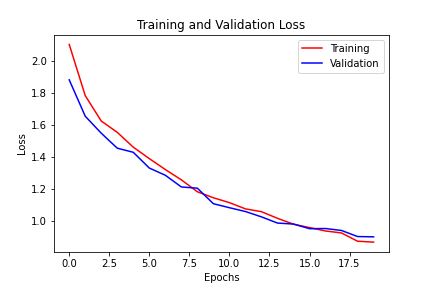
\includegraphics[width=0.5\textwidth,height=.3\textheight]{4_LossFedAvgM_iid.png}
    \caption{Loss using FedAvgM with iid data distributions}
     \label{LossFedAvgMIid} 
\end{figure}

An attempt was made to see if the behaviour changed for different values of momentum . The plots of accuracies in figure \ref{AccFedAvgB0.7} and in figure \ref{AccFedAvgB0.997} show that when beta is lower the number of oscillations is higher, and their height is bigger.
\begin{figure}
    \centering
    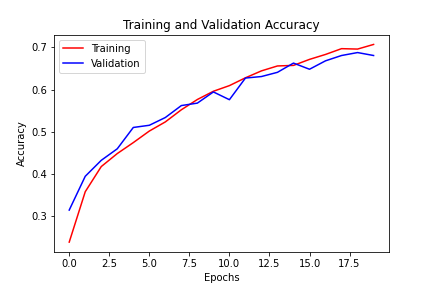
\includegraphics[width=0.5\textwidth,height=.3\textheight]{5_AccuracyFedAvgM_Beta0.7.png}
    \caption{Accuracy using FedAvgM with Beta = 0.7}
     \label{AccFedAvgB0.7} 
\end{figure}

\begin{figure}
    \centering
    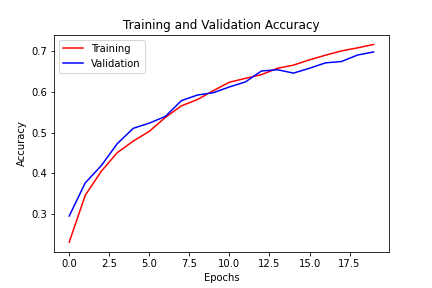
\includegraphics[width=0.5\textwidth,height=.3\textheight]{5_AccuracyFedAvgM_Beta0.997.png}
    \caption{Accuracy using FedAvgM with Beta = 0.997}
     \label{AccFedAvgB0.997} 
\end{figure}

With the non-IID data distributions for the clients, the results are slightly better than vanilla FedAvg's ones. 

\begin{figure}
    \centering
    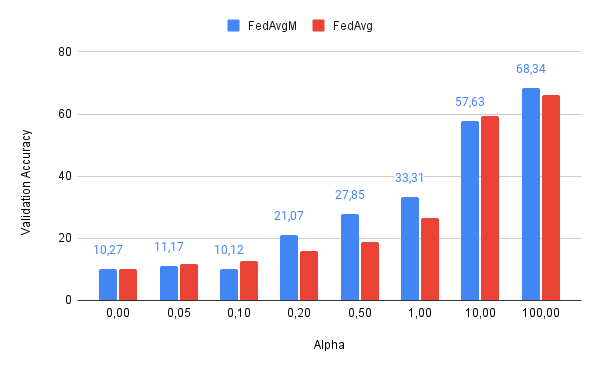
\includegraphics[width=0.5\textwidth,height=.3\textheight]{FedAvgMvsFedAvg.png}
    \caption{Accuracy comparison between FedAvg and FedAvgMomentum}
    \label{FedAvgvsFedM} 
\end{figure}

However, even in this case, there is a large presence of oscillations, particularly for small values of alpha, which makes comparison difficult.
We can see that from figures \ref{AccFedAvgMA1} , \ref{AccFedAvgMA10} and \ref{AccFedAvgMA100}.


\begin{figure}
    \centering
    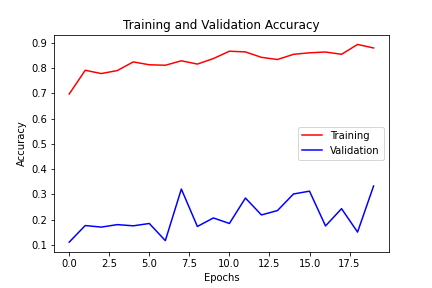
\includegraphics[width=0.5\textwidth,height=.3\textheight]{7_AccuracyFedAvgM_A1.png}
    \caption{Accuracy using FedAvgM with Alpha = 1}
     \label{AccFedAvgMA1} 
\end{figure}

\begin{figure}
    \centering
    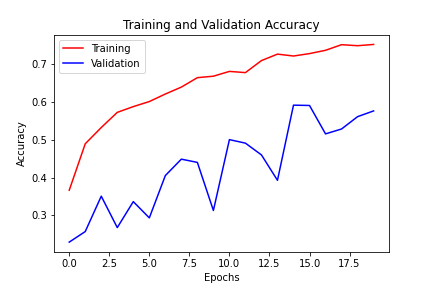
\includegraphics[width=0.5\textwidth,height=.3\textheight]{7_AccuracyFedAvgM_A10.png}
    \caption{Accuracy using FedAvgM with Alpha = 10}
     \label{AccFedAvgMA10} 
\end{figure}

\begin{figure}
    \centering
    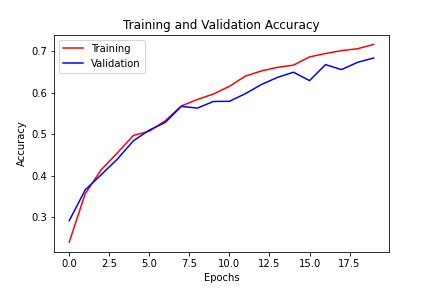
\includegraphics[width=0.5\textwidth,height=.3\textheight]{7_AccuracyFedAvgM_A100.png}
    \caption{Accuracy using FedAvgM with Alpha = 100}
     \label{AccFedAvgMA100} 
\end{figure}


Since in the original setting the number of rounds is too low to appreciate any major difference between the vanilla FedAvg and FedAvgM behaviors, a decision was taken to change the setup by increasing the number of rounds to 1000, and decreasing the number of local epochs to 1 so that the computation could still be handled by the system.
The idea was to explore different regions where data distribution would differs, making reference to paper \cite{DBLP:journals/corr/KonecnyMYRSB16}.


In the case with Alpha = 1 both the models reached accuracy around 0.7 and their trend is very similar, with wide oscillations in particular at the beginning.

\begin{figure}
    \centering
    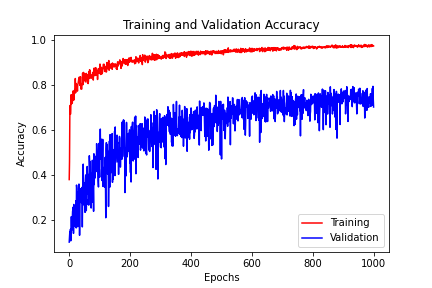
\includegraphics[width=0.5\textwidth,height=.3\textheight]{9_AccuracyFedAvg_C0.3A_1.png}
    \caption{Accuracy using FedAvg with C = 0.3 and Alpha = 1}
     \label{AccFedAvgC0.3A1} 
\end{figure}

\begin{figure}
    \centering
    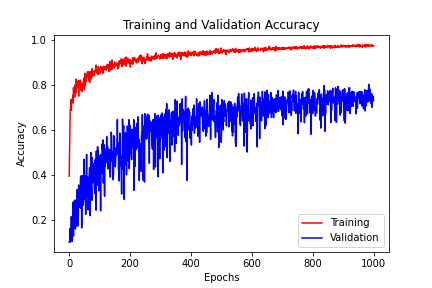
\includegraphics[width=0.5\textwidth,height=.3\textheight]{9_AccuracyFedAvgM_C0.3A_1.png}
    \caption{Accuracy using FedAvgM with C = 0.3 and Alpha = 1}
     \label{AccFedAvgMC0.3A1} 
\end{figure}

Then another attempt was made to pick a case where the differences would be more evident changing Alpha to 0.05, and additionally changing the percentage of selected clients at each round (C) from 0.3 to 0.1. 
However, even on this occasion, as shown in figure \ref{AccFedAvgC0.1A0.05} and in figure \ref{AccFedAvgMC0.1A0.05}, the two algorithms achieve similar results. In this case FedAvgM's algorithm fails to achieve the expected accuracy. Probably with such low values of Alpha it would take an even greater number of rounds, which was not possible to test due to the limitations of the hardware at hand. The major difference between the two plots is at the beginning, where FedAvg starts with a higher value of training accuracy and converges faster.

\begin{figure}
    \centering
    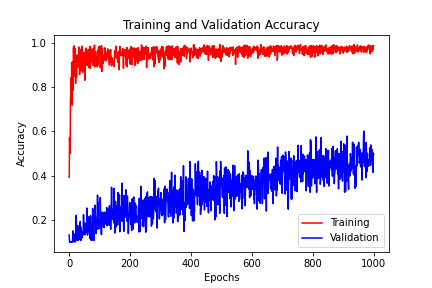
\includegraphics[width=0.5\textwidth,height=.3\textheight]{10_AccuracyFedAvg_C0.1A_0.05.png}
    \caption{Accuracy using FedAvg with C = 0.1 and Alpha = 0.05}
     \label{AccFedAvgC0.1A0.05} 
\end{figure}

\begin{figure}
    \centering
    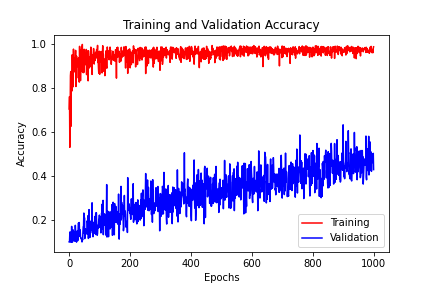
\includegraphics[width=0.5\textwidth,height=.3\textheight]{10_AccuracyFedAvgM_C0.1_A0.05.png}
    \caption{Accuracy using FedAvgM with C = 0.1 and Alpha = 0.05}
     \label{AccFedAvgMC0.1A0.05} 
\end{figure}





\subsection{Conclusion}
The general idea that can be drawn from this work is that, although it doesn't have the accuracy of the centralised model, Federated Learning works and can be used on real life scenarios.

Moreover, as it has been shown with, the FedAvg does just fine if not fine tuned, and certainly normalization helps to improve the accuracy. As a general tendency, the normalization improves the  accuracy, whether it is group or batch normalization (even though group normalization has better performances). 

Additionally, the introduction of non IID and different quantity of data to the clients increased the difficulty of data treatment and learning. However, if the parameters didn't led to extreme cases, the accuracy was still acceptable.

Finally, in order to deal with the non IID, the FedAvgMomentum, at first was thought as a feasible solution to improve the accuracy, however, the algorithm ended up not having the positive impact expected with the resources that were available.

\printbibliography

\end{document}
